\documentclass[12pt]{article}
\usepackage{tikz}
\usepackage{amsmath}
% Underlining package
\usepackage{ulem}
\usetikzlibrary{calc}
\usetikzlibrary{angles,quotes}
\usepackage[a4paper, portrait, margin=1cm]{geometry}
\usepackage{fancyhdr}

\newcommand{\HeadingAnswers}{%
\section*{\Large Name: \underline{\hspace{8cm}} \hfill Date: \underline{\hspace{3cm}}}%
\vspace{-3mm}\par
\textbf{Area Squares: Answers}\vspace{1pt}\hrule
}

% raise footer with page number; no header
\fancypagestyle{myfancypagestyle}{
  \fancyhf{}% clear all header and footer fields
  \renewcommand{\headrulewidth}{0pt} % no rule under header
  \fancyfoot[C] {\thepage} \setlength{\footskip}{14.5pt} % raise page number allowed min 14.5pt
}
\pagestyle{myfancypagestyle}  % apply myfancypagestyle

\newcounter{minipagecount}

\begin{document}
\HeadingAnswers
\vspace{8mm}

\begin{minipage}{0.55\textwidth}
  \refstepcounter{minipagecount}
  \noindent{(\theminipagecount)}\quad
  \begin{tikzpicture}[scale=1.1, baseline=(current bounding box.north)]
    \begin{scope}[rotate=0]
        % Draw square
        \draw (0,0) coordinate (Q) --
              ++(2.916,0) coordinate (R) --
              ++(0,2.916) coordinate (S) --
              ++(-2.916,0) coordinate (T) -- cycle;

        % Right angle markers
        \foreach \p/\q/\r in {T/Q/R,Q/R/S,S/T/Q,T/Q/R} {
            \pic [draw, -, angle radius=0.2cm] {right angle=\p--\q--\r};
        }

        % Vertex LABELS
        \foreach \p/\l in {Q/below left,R/below right,S/above right,T/above left} {
            \node[\l] at (\p) {\p};
        }

        % Dotted arrows shifted away from edges
        % Horizontal side (A-B), shifted down
        \draw[<->, dotted]
            ($(Q) + (0,-0.2cm)$) -- ($(R) + (0,-0.2cm)$)
            node[midway,below, xshift=2mm] {3\,cm};

        % Vertical side (B-C), shifted right
        \draw[<->, dotted]
            ($(R) + (0.2cm,0)$) -- ($(S) + (0.2cm,0)$)
            node[midway,right] {3\,cm};
    \end{scope}
\end{tikzpicture}
\end{minipage}%
\hfill
\begin{minipage}{.4\textwidth}
  \begin{align*}
  \text{Area} &= l^2 \\
  \text{Area} &= 3 \,\text{cm} \times 3 \,\text{cm} \\
  \text{Area} &= 9 \,\text{cm}^2
  \end{align*}
\end{minipage}
\par\vspace{1cm}\begin{minipage}{0.55\textwidth}
  \refstepcounter{minipagecount}
  \noindent{(\theminipagecount)}\quad
  \begin{tikzpicture}[scale=1.1, baseline=(current bounding box.north)]
    \begin{scope}[rotate=0]
        % Draw square
        \draw (0,0) coordinate (K) --
              ++(1.939,0) coordinate (L) --
              ++(0,1.939) coordinate (M) --
              ++(-1.939,0) coordinate (N) -- cycle;

        % Right angle markers
        \foreach \p/\q/\r in {N/K/L,K/L/M,M/N/K,N/K/L} {
            \pic [draw, -, angle radius=0.2cm] {right angle=\p--\q--\r};
        }

        % Vertex LABELS
        \foreach \p/\l in {K/below left,L/below right,M/above right,N/above left} {
            \node[\l] at (\p) {\p};
        }

        % Dotted arrows shifted away from edges
        % Horizontal side (A-B), shifted down
        \draw[<->, dotted]
            ($(K) + (0,-0.2cm)$) -- ($(L) + (0,-0.2cm)$)
            node[midway,below, xshift=2mm] {7\,cm};

        % Vertical side (B-C), shifted right
        \draw[<->, dotted]
            ($(L) + (0.2cm,0)$) -- ($(M) + (0.2cm,0)$)
            node[midway,right] {7\,cm};
    \end{scope}
\end{tikzpicture}
\end{minipage}%
\hfill
\begin{minipage}{.4\textwidth}
  \begin{align*}
  \text{Area} &= l^2 \\
  \text{Area} &= 7 \,\text{cm} \times 7 \,\text{cm} \\
  \text{Area} &= 49 \,\text{cm}^2
  \end{align*}
\end{minipage}
\par\vspace{1cm}\begin{minipage}{0.55\textwidth}
  \refstepcounter{minipagecount}
  \noindent{(\theminipagecount)}\quad
  \begin{tikzpicture}[scale=1.1, baseline=(current bounding box.north)]
    \begin{scope}[rotate=0]
        % Draw square
        \draw (0,0) coordinate (A) --
              ++(2.784,0) coordinate (B) --
              ++(0,2.784) coordinate (C) --
              ++(-2.784,0) coordinate (D) -- cycle;

        % Right angle markers
        \foreach \p/\q/\r in {D/A/B,A/B/C,C/D/A,D/A/B} {
            \pic [draw, -, angle radius=0.2cm] {right angle=\p--\q--\r};
        }

        % Vertex LABELS
        \foreach \p/\l in {A/below left,B/below right,C/above right,D/above left} {
            \node[\l] at (\p) {\p};
        }

        % Dotted arrows shifted away from edges
        % Horizontal side (A-B), shifted down
        \draw[<->, dotted]
            ($(A) + (0,-0.2cm)$) -- ($(B) + (0,-0.2cm)$)
            node[midway,below, xshift=2mm] {1\,cm};

        % Vertical side (B-C), shifted right
        \draw[<->, dotted]
            ($(B) + (0.2cm,0)$) -- ($(C) + (0.2cm,0)$)
            node[midway,right] {1\,cm};
    \end{scope}
\end{tikzpicture}
\end{minipage}%
\hfill
\begin{minipage}{.4\textwidth}
  \begin{align*}
  \text{Area} &= l^2 \\
  \text{Area} &= 1 \,\text{cm} \times 1 \,\text{cm} \\
  \text{Area} &= 1 \,\text{cm}^2
  \end{align*}
\end{minipage}
\par\vspace{1cm}\begin{minipage}{0.55\textwidth}
  \refstepcounter{minipagecount}
  \noindent{(\theminipagecount)}\quad
  \begin{tikzpicture}[scale=1.1, baseline=(current bounding box.north)]
    \begin{scope}[rotate=0]
        % Draw square
        \draw (0,0) coordinate (Q) --
              ++(2.4,0) coordinate (R) --
              ++(0,2.4) coordinate (S) --
              ++(-2.4,0) coordinate (T) -- cycle;

        % Right angle markers
        \foreach \p/\q/\r in {T/Q/R,Q/R/S,S/T/Q,T/Q/R} {
            \pic [draw, -, angle radius=0.2cm] {right angle=\p--\q--\r};
        }

        % Vertex LABELS
        \foreach \p/\l in {Q/below left,R/below right,S/above right,T/above left} {
            \node[\l] at (\p) {\p};
        }

        % Dotted arrows shifted away from edges
        % Horizontal side (A-B), shifted down
        \draw[<->, dotted]
            ($(Q) + (0,-0.2cm)$) -- ($(R) + (0,-0.2cm)$)
            node[midway,below, xshift=2mm] {8\,cm};

        % Vertical side (B-C), shifted right
        \draw[<->, dotted]
            ($(R) + (0.2cm,0)$) -- ($(S) + (0.2cm,0)$)
            node[midway,right] {8\,cm};
    \end{scope}
\end{tikzpicture}
\end{minipage}%
\hfill
\begin{minipage}{.4\textwidth}
  \begin{align*}
  \text{Area} &= l^2 \\
  \text{Area} &= 8 \,\text{cm} \times 8 \,\text{cm} \\
  \text{Area} &= 64 \,\text{cm}^2
  \end{align*}
\end{minipage}
\par\vspace{1cm}\begin{minipage}{0.55\textwidth}
  \refstepcounter{minipagecount}
  \noindent{(\theminipagecount)}\quad
  \begin{tikzpicture}[scale=1.1, baseline=(current bounding box.north)]
    \begin{scope}[rotate=0]
        % Draw square
        \draw (0,0) coordinate (Q) --
              ++(2.994,0) coordinate (R) --
              ++(0,2.994) coordinate (S) --
              ++(-2.994,0) coordinate (T) -- cycle;

        % Right angle markers
        \foreach \p/\q/\r in {T/Q/R,Q/R/S,S/T/Q,T/Q/R} {
            \pic [draw, -, angle radius=0.2cm] {right angle=\p--\q--\r};
        }

        % Vertex LABELS
        \foreach \p/\l in {Q/below left,R/below right,S/above right,T/above left} {
            \node[\l] at (\p) {\p};
        }

        % Dotted arrows shifted away from edges
        % Horizontal side (A-B), shifted down
        \draw[<->, dotted]
            ($(Q) + (0,-0.2cm)$) -- ($(R) + (0,-0.2cm)$)
            node[midway,below, xshift=2mm] {9\,cm};

        % Vertical side (B-C), shifted right
        \draw[<->, dotted]
            ($(R) + (0.2cm,0)$) -- ($(S) + (0.2cm,0)$)
            node[midway,right] {9\,cm};
    \end{scope}
\end{tikzpicture}
\end{minipage}%
\hfill
\begin{minipage}{.4\textwidth}
  \begin{align*}
  \text{Area} &= l^2 \\
  \text{Area} &= 9 \,\text{cm} \times 9 \,\text{cm} \\
  \text{Area} &= 81 \,\text{cm}^2
  \end{align*}
\end{minipage}
\par\vspace{1cm}\begin{minipage}{0.55\textwidth}
  \refstepcounter{minipagecount}
  \noindent{(\theminipagecount)}\quad
  \begin{tikzpicture}[scale=1.1, baseline=(current bounding box.north)]
    \begin{scope}[rotate=0]
        % Draw square
        \draw (0,0) coordinate (W) --
              ++(2.374,0) coordinate (X) --
              ++(0,2.374) coordinate (Y) --
              ++(-2.374,0) coordinate (Z) -- cycle;

        % Right angle markers
        \foreach \p/\q/\r in {Z/W/X,W/X/Y,Y/Z/W,Z/W/X} {
            \pic [draw, -, angle radius=0.2cm] {right angle=\p--\q--\r};
        }

        % Vertex LABELS
        \foreach \p/\l in {W/below left,X/below right,Y/above right,Z/above left} {
            \node[\l] at (\p) {\p};
        }

        % Dotted arrows shifted away from edges
        % Horizontal side (A-B), shifted down
        \draw[<->, dotted]
            ($(W) + (0,-0.2cm)$) -- ($(X) + (0,-0.2cm)$)
            node[midway,below, xshift=2mm] {4\,cm};

        % Vertical side (B-C), shifted right
        \draw[<->, dotted]
            ($(X) + (0.2cm,0)$) -- ($(Y) + (0.2cm,0)$)
            node[midway,right] {4\,cm};
    \end{scope}
\end{tikzpicture}
\end{minipage}%
\hfill
\begin{minipage}{.4\textwidth}
  \begin{align*}
  \text{Area} &= l^2 \\
  \text{Area} &= 4 \,\text{cm} \times 4 \,\text{cm} \\
  \text{Area} &= 16 \,\text{cm}^2
  \end{align*}
\end{minipage}
\par\vspace{1cm}\begin{minipage}{0.55\textwidth}
  \refstepcounter{minipagecount}
  \noindent{(\theminipagecount)}\quad
  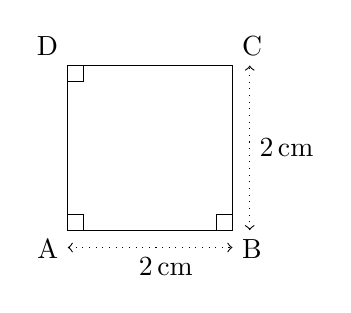
\begin{tikzpicture}[scale=1.1, baseline=(current bounding box.north)]
    \begin{scope}[rotate=0]
        % Draw square
        \draw (0,0) coordinate (A) --
              ++(1.9,0) coordinate (B) --
              ++(0,1.9) coordinate (C) --
              ++(-1.9,0) coordinate (D) -- cycle;

        % Right angle markers
        \foreach \p/\q/\r in {D/A/B,A/B/C,C/D/A,D/A/B} {
            \pic [draw, -, angle radius=0.2cm] {right angle=\p--\q--\r};
        }

        % Vertex LABELS
        \foreach \p/\l in {A/below left,B/below right,C/above right,D/above left} {
            \node[\l] at (\p) {\p};
        }

        % Dotted arrows shifted away from edges
        % Horizontal side (A-B), shifted down
        \draw[<->, dotted]
            ($(A) + (0,-0.2cm)$) -- ($(B) + (0,-0.2cm)$)
            node[midway,below, xshift=2mm] {2\,cm};

        % Vertical side (B-C), shifted right
        \draw[<->, dotted]
            ($(B) + (0.2cm,0)$) -- ($(C) + (0.2cm,0)$)
            node[midway,right] {2\,cm};
    \end{scope}
\end{tikzpicture}
\end{minipage}%
\hfill
\begin{minipage}{.4\textwidth}
  \begin{align*}
  \text{Area} &= l^2 \\
  \text{Area} &= 2 \,\text{cm} \times 2 \,\text{cm} \\
  \text{Area} &= 4 \,\text{cm}^2
  \end{align*}
\end{minipage}
\par\vspace{1cm}\begin{minipage}{0.55\textwidth}
  \refstepcounter{minipagecount}
  \noindent{(\theminipagecount)}\quad
  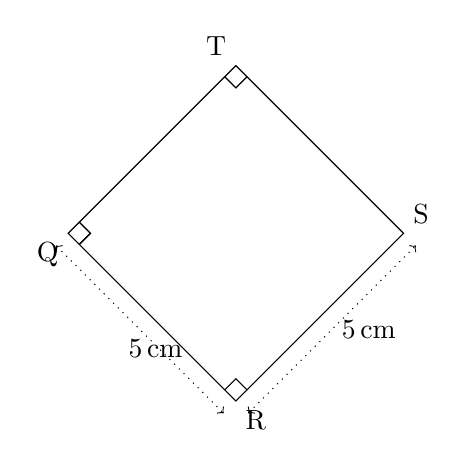
\begin{tikzpicture}[scale=1.1, baseline=(current bounding box.north)]
    \begin{scope}[rotate=-45]
        % Draw square
        \draw (0,0) coordinate (Q) --
              ++(2.738,0) coordinate (R) --
              ++(0,2.738) coordinate (S) --
              ++(-2.738,0) coordinate (T) -- cycle;

        % Right angle markers
        \foreach \p/\q/\r in {T/Q/R,Q/R/S,S/T/Q,T/Q/R} {
            \pic [draw, -, angle radius=0.2cm] {right angle=\p--\q--\r};
        }

        % Vertex LABELS
        \foreach \p/\l in {Q/below left,R/below right,S/above right,T/above left} {
            \node[\l] at (\p) {\p};
        }

        % Dotted arrows shifted away from edges
        % Horizontal side (A-B), shifted down
        \draw[<->, dotted]
            ($(Q) + (0,-0.2cm)$) -- ($(R) + (0,-0.2cm)$)
            node[midway,below, xshift=2mm] {5\,cm};

        % Vertical side (B-C), shifted right
        \draw[<->, dotted]
            ($(R) + (0.2cm,0)$) -- ($(S) + (0.2cm,0)$)
            node[midway,right] {5\,cm};
    \end{scope}
\end{tikzpicture}
\end{minipage}%
\hfill
\begin{minipage}{.4\textwidth}
  \begin{align*}
  \text{Area} &= l^2 \\
  \text{Area} &= 5 \,\text{cm} \times 5 \,\text{cm} \\
  \text{Area} &= 25 \,\text{cm}^2
  \end{align*}
\end{minipage}
\par\vspace{1cm}\begin{minipage}{0.55\textwidth}
  \refstepcounter{minipagecount}
  \noindent{(\theminipagecount)}\quad
  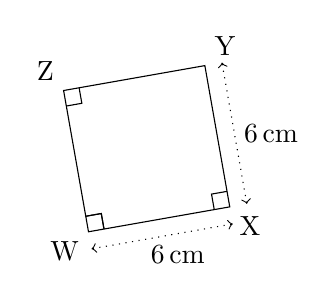
\begin{tikzpicture}[scale=1.1, baseline=(current bounding box.north)]
    \begin{scope}[rotate=10]
        % Draw square
        \draw (0,0) coordinate (W) --
              ++(1.656,0) coordinate (X) --
              ++(0,1.656) coordinate (Y) --
              ++(-1.656,0) coordinate (Z) -- cycle;

        % Right angle markers
        \foreach \p/\q/\r in {Z/W/X,W/X/Y,Y/Z/W,Z/W/X} {
            \pic [draw, -, angle radius=0.2cm] {right angle=\p--\q--\r};
        }

        % Vertex LABELS
        \foreach \p/\l in {W/below left,X/below right,Y/above right,Z/above left} {
            \node[\l] at (\p) {\p};
        }

        % Dotted arrows shifted away from edges
        % Horizontal side (A-B), shifted down
        \draw[<->, dotted]
            ($(W) + (0,-0.2cm)$) -- ($(X) + (0,-0.2cm)$)
            node[midway,below, xshift=2mm] {6\,cm};

        % Vertical side (B-C), shifted right
        \draw[<->, dotted]
            ($(X) + (0.2cm,0)$) -- ($(Y) + (0.2cm,0)$)
            node[midway,right] {6\,cm};
    \end{scope}
\end{tikzpicture}
\end{minipage}%
\hfill
\begin{minipage}{.4\textwidth}
  \begin{align*}
  \text{Area} &= l^2 \\
  \text{Area} &= 6 \,\text{cm} \times 6 \,\text{cm} \\
  \text{Area} &= 36 \,\text{cm}^2
  \end{align*}
\end{minipage}
\par\vspace{1cm}\begin{minipage}{0.55\textwidth}
  \refstepcounter{minipagecount}
  \noindent{(\theminipagecount)}\quad
  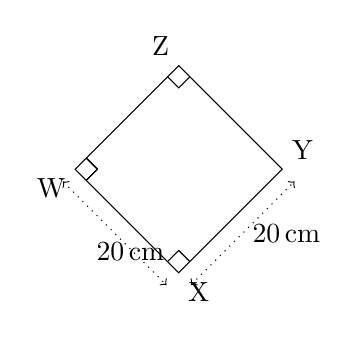
\begin{tikzpicture}[scale=1.1, baseline=(current bounding box.north)]
    \begin{scope}[rotate=-45]
        % Draw square
        \draw (0,0) coordinate (W) --
              ++(1.691,0) coordinate (X) --
              ++(0,1.691) coordinate (Y) --
              ++(-1.691,0) coordinate (Z) -- cycle;

        % Right angle markers
        \foreach \p/\q/\r in {Z/W/X,W/X/Y,Y/Z/W,Z/W/X} {
            \pic [draw, -, angle radius=0.2cm] {right angle=\p--\q--\r};
        }

        % Vertex LABELS
        \foreach \p/\l in {W/below left,X/below right,Y/above right,Z/above left} {
            \node[\l] at (\p) {\p};
        }

        % Dotted arrows shifted away from edges
        % Horizontal side (A-B), shifted down
        \draw[<->, dotted]
            ($(W) + (0,-0.2cm)$) -- ($(X) + (0,-0.2cm)$)
            node[midway,below, xshift=2mm] {20\,cm};

        % Vertical side (B-C), shifted right
        \draw[<->, dotted]
            ($(X) + (0.2cm,0)$) -- ($(Y) + (0.2cm,0)$)
            node[midway,right] {20\,cm};
    \end{scope}
\end{tikzpicture}
\end{minipage}%
\hfill
\begin{minipage}{.4\textwidth}
  \begin{align*}
  \text{Area} &= l^2 \\
  \text{Area} &= 20 \,\text{cm} \times 20 \,\text{cm} \\
  \text{Area} &= 400 \,\text{cm}^2
  \end{align*}
\end{minipage}
\par\vspace{1cm}\begin{minipage}{0.55\textwidth}
  \refstepcounter{minipagecount}
  \noindent{(\theminipagecount)}\quad
  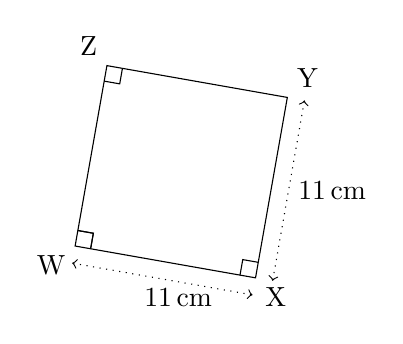
\begin{tikzpicture}[scale=1.1, baseline=(current bounding box.north)]
    \begin{scope}[rotate=-10]
        % Draw square
        \draw (0,0) coordinate (W) --
              ++(2.115,0) coordinate (X) --
              ++(0,2.115) coordinate (Y) --
              ++(-2.115,0) coordinate (Z) -- cycle;

        % Right angle markers
        \foreach \p/\q/\r in {Z/W/X,W/X/Y,Y/Z/W,Z/W/X} {
            \pic [draw, -, angle radius=0.2cm] {right angle=\p--\q--\r};
        }

        % Vertex LABELS
        \foreach \p/\l in {W/below left,X/below right,Y/above right,Z/above left} {
            \node[\l] at (\p) {\p};
        }

        % Dotted arrows shifted away from edges
        % Horizontal side (A-B), shifted down
        \draw[<->, dotted]
            ($(W) + (0,-0.2cm)$) -- ($(X) + (0,-0.2cm)$)
            node[midway,below, xshift=2mm] {11\,cm};

        % Vertical side (B-C), shifted right
        \draw[<->, dotted]
            ($(X) + (0.2cm,0)$) -- ($(Y) + (0.2cm,0)$)
            node[midway,right] {11\,cm};
    \end{scope}
\end{tikzpicture}
\end{minipage}%
\hfill
\begin{minipage}{.4\textwidth}
  \begin{align*}
  \text{Area} &= l^2 \\
  \text{Area} &= 11 \,\text{cm} \times 11 \,\text{cm} \\
  \text{Area} &= 121 \,\text{cm}^2
  \end{align*}
\end{minipage}
\par\vspace{1cm}\begin{minipage}{0.55\textwidth}
  \refstepcounter{minipagecount}
  \noindent{(\theminipagecount)}\quad
  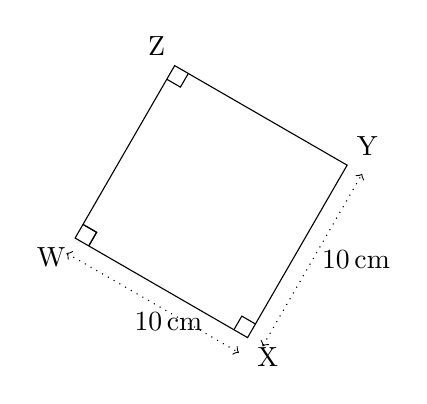
\begin{tikzpicture}[scale=1.1, baseline=(current bounding box.north)]
    \begin{scope}[rotate=-30]
        % Draw square
        \draw (0,0) coordinate (W) --
              ++(2.299,0) coordinate (X) --
              ++(0,2.299) coordinate (Y) --
              ++(-2.299,0) coordinate (Z) -- cycle;

        % Right angle markers
        \foreach \p/\q/\r in {Z/W/X,W/X/Y,Y/Z/W,Z/W/X} {
            \pic [draw, -, angle radius=0.2cm] {right angle=\p--\q--\r};
        }

        % Vertex LABELS
        \foreach \p/\l in {W/below left,X/below right,Y/above right,Z/above left} {
            \node[\l] at (\p) {\p};
        }

        % Dotted arrows shifted away from edges
        % Horizontal side (A-B), shifted down
        \draw[<->, dotted]
            ($(W) + (0,-0.2cm)$) -- ($(X) + (0,-0.2cm)$)
            node[midway,below, xshift=2mm] {10\,cm};

        % Vertical side (B-C), shifted right
        \draw[<->, dotted]
            ($(X) + (0.2cm,0)$) -- ($(Y) + (0.2cm,0)$)
            node[midway,right] {10\,cm};
    \end{scope}
\end{tikzpicture}
\end{minipage}%
\hfill
\begin{minipage}{.4\textwidth}
  \begin{align*}
  \text{Area} &= l^2 \\
  \text{Area} &= 10 \,\text{cm} \times 10 \,\text{cm} \\
  \text{Area} &= 100 \,\text{cm}^2
  \end{align*}
\end{minipage}
\par\vspace{1cm}\begin{minipage}{0.55\textwidth}
  \refstepcounter{minipagecount}
  \noindent{(\theminipagecount)}\quad
  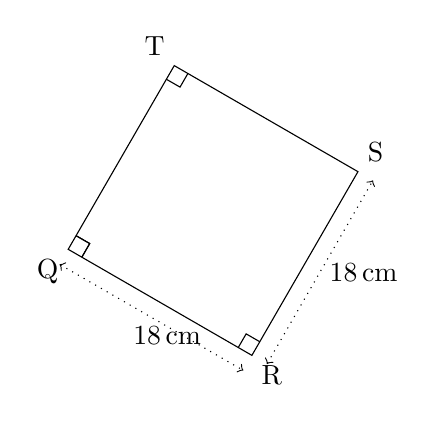
\begin{tikzpicture}[scale=1.1, baseline=(current bounding box.north)]
    \begin{scope}[rotate=-30]
        % Draw square
        \draw (0,0) coordinate (Q) --
              ++(2.449,0) coordinate (R) --
              ++(0,2.449) coordinate (S) --
              ++(-2.449,0) coordinate (T) -- cycle;

        % Right angle markers
        \foreach \p/\q/\r in {T/Q/R,Q/R/S,S/T/Q,T/Q/R} {
            \pic [draw, -, angle radius=0.2cm] {right angle=\p--\q--\r};
        }

        % Vertex LABELS
        \foreach \p/\l in {Q/below left,R/below right,S/above right,T/above left} {
            \node[\l] at (\p) {\p};
        }

        % Dotted arrows shifted away from edges
        % Horizontal side (A-B), shifted down
        \draw[<->, dotted]
            ($(Q) + (0,-0.2cm)$) -- ($(R) + (0,-0.2cm)$)
            node[midway,below, xshift=2mm] {18\,cm};

        % Vertical side (B-C), shifted right
        \draw[<->, dotted]
            ($(R) + (0.2cm,0)$) -- ($(S) + (0.2cm,0)$)
            node[midway,right] {18\,cm};
    \end{scope}
\end{tikzpicture}
\end{minipage}%
\hfill
\begin{minipage}{.4\textwidth}
  \begin{align*}
  \text{Area} &= l^2 \\
  \text{Area} &= 18 \,\text{cm} \times 18 \,\text{cm} \\
  \text{Area} &= 324 \,\text{cm}^2
  \end{align*}
\end{minipage}
\par\vspace{1cm}\begin{minipage}{0.55\textwidth}
  \refstepcounter{minipagecount}
  \noindent{(\theminipagecount)}\quad
  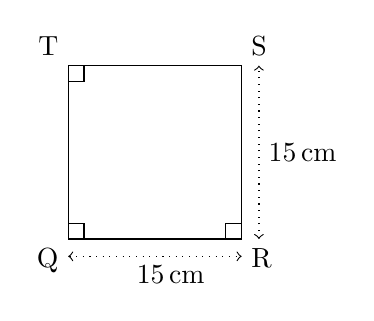
\begin{tikzpicture}[scale=1.1, baseline=(current bounding box.north)]
    \begin{scope}[rotate=0]
        % Draw square
        \draw (0,0) coordinate (Q) --
              ++(2.002,0) coordinate (R) --
              ++(0,2.002) coordinate (S) --
              ++(-2.002,0) coordinate (T) -- cycle;

        % Right angle markers
        \foreach \p/\q/\r in {T/Q/R,Q/R/S,S/T/Q,T/Q/R} {
            \pic [draw, -, angle radius=0.2cm] {right angle=\p--\q--\r};
        }

        % Vertex LABELS
        \foreach \p/\l in {Q/below left,R/below right,S/above right,T/above left} {
            \node[\l] at (\p) {\p};
        }

        % Dotted arrows shifted away from edges
        % Horizontal side (A-B), shifted down
        \draw[<->, dotted]
            ($(Q) + (0,-0.2cm)$) -- ($(R) + (0,-0.2cm)$)
            node[midway,below, xshift=2mm] {15\,cm};

        % Vertical side (B-C), shifted right
        \draw[<->, dotted]
            ($(R) + (0.2cm,0)$) -- ($(S) + (0.2cm,0)$)
            node[midway,right] {15\,cm};
    \end{scope}
\end{tikzpicture}
\end{minipage}%
\hfill
\begin{minipage}{.4\textwidth}
  \begin{align*}
  \text{Area} &= l^2 \\
  \text{Area} &= 15 \,\text{cm} \times 15 \,\text{cm} \\
  \text{Area} &= 225 \,\text{cm}^2
  \end{align*}
\end{minipage}
\par\vspace{1cm}\begin{minipage}{0.55\textwidth}
  \refstepcounter{minipagecount}
  \noindent{(\theminipagecount)}\quad
  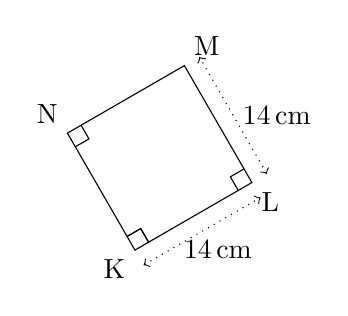
\begin{tikzpicture}[scale=1.1, baseline=(current bounding box.north)]
    \begin{scope}[rotate=30]
        % Draw square
        \draw (0,0) coordinate (K) --
              ++(1.559,0) coordinate (L) --
              ++(0,1.559) coordinate (M) --
              ++(-1.559,0) coordinate (N) -- cycle;

        % Right angle markers
        \foreach \p/\q/\r in {N/K/L,K/L/M,M/N/K,N/K/L} {
            \pic [draw, -, angle radius=0.2cm] {right angle=\p--\q--\r};
        }

        % Vertex LABELS
        \foreach \p/\l in {K/below left,L/below right,M/above right,N/above left} {
            \node[\l] at (\p) {\p};
        }

        % Dotted arrows shifted away from edges
        % Horizontal side (A-B), shifted down
        \draw[<->, dotted]
            ($(K) + (0,-0.2cm)$) -- ($(L) + (0,-0.2cm)$)
            node[midway,below, xshift=2mm] {14\,cm};

        % Vertical side (B-C), shifted right
        \draw[<->, dotted]
            ($(L) + (0.2cm,0)$) -- ($(M) + (0.2cm,0)$)
            node[midway,right] {14\,cm};
    \end{scope}
\end{tikzpicture}
\end{minipage}%
\hfill
\begin{minipage}{.4\textwidth}
  \begin{align*}
  \text{Area} &= l^2 \\
  \text{Area} &= 14 \,\text{cm} \times 14 \,\text{cm} \\
  \text{Area} &= 196 \,\text{cm}^2
  \end{align*}
\end{minipage}
\par\vspace{1cm}\begin{minipage}{0.55\textwidth}
  \refstepcounter{minipagecount}
  \noindent{(\theminipagecount)}\quad
  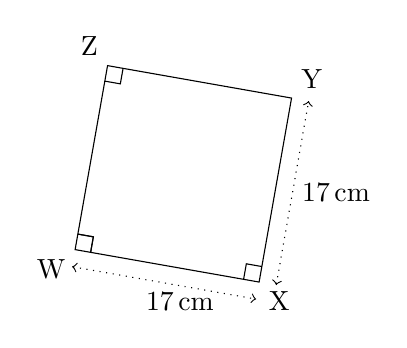
\begin{tikzpicture}[scale=1.1, baseline=(current bounding box.north)]
    \begin{scope}[rotate=-10]
        % Draw square
        \draw (0,0) coordinate (W) --
              ++(2.157,0) coordinate (X) --
              ++(0,2.157) coordinate (Y) --
              ++(-2.157,0) coordinate (Z) -- cycle;

        % Right angle markers
        \foreach \p/\q/\r in {Z/W/X,W/X/Y,Y/Z/W,Z/W/X} {
            \pic [draw, -, angle radius=0.2cm] {right angle=\p--\q--\r};
        }

        % Vertex LABELS
        \foreach \p/\l in {W/below left,X/below right,Y/above right,Z/above left} {
            \node[\l] at (\p) {\p};
        }

        % Dotted arrows shifted away from edges
        % Horizontal side (A-B), shifted down
        \draw[<->, dotted]
            ($(W) + (0,-0.2cm)$) -- ($(X) + (0,-0.2cm)$)
            node[midway,below, xshift=2mm] {17\,cm};

        % Vertical side (B-C), shifted right
        \draw[<->, dotted]
            ($(X) + (0.2cm,0)$) -- ($(Y) + (0.2cm,0)$)
            node[midway,right] {17\,cm};
    \end{scope}
\end{tikzpicture}
\end{minipage}%
\hfill
\begin{minipage}{.4\textwidth}
  \begin{align*}
  \text{Area} &= l^2 \\
  \text{Area} &= 17 \,\text{cm} \times 17 \,\text{cm} \\
  \text{Area} &= 289 \,\text{cm}^2
  \end{align*}
\end{minipage}
\par\vspace{1cm}\begin{minipage}{0.55\textwidth}
  \refstepcounter{minipagecount}
  \noindent{(\theminipagecount)}\quad
  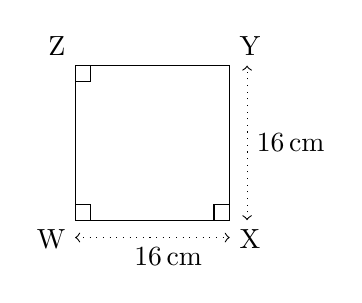
\begin{tikzpicture}[scale=1.1, baseline=(current bounding box.north)]
    \begin{scope}[rotate=0]
        % Draw square
        \draw (0,0) coordinate (W) --
              ++(1.785,0) coordinate (X) --
              ++(0,1.785) coordinate (Y) --
              ++(-1.785,0) coordinate (Z) -- cycle;

        % Right angle markers
        \foreach \p/\q/\r in {Z/W/X,W/X/Y,Y/Z/W,Z/W/X} {
            \pic [draw, -, angle radius=0.2cm] {right angle=\p--\q--\r};
        }

        % Vertex LABELS
        \foreach \p/\l in {W/below left,X/below right,Y/above right,Z/above left} {
            \node[\l] at (\p) {\p};
        }

        % Dotted arrows shifted away from edges
        % Horizontal side (A-B), shifted down
        \draw[<->, dotted]
            ($(W) + (0,-0.2cm)$) -- ($(X) + (0,-0.2cm)$)
            node[midway,below, xshift=2mm] {16\,cm};

        % Vertical side (B-C), shifted right
        \draw[<->, dotted]
            ($(X) + (0.2cm,0)$) -- ($(Y) + (0.2cm,0)$)
            node[midway,right] {16\,cm};
    \end{scope}
\end{tikzpicture}
\end{minipage}%
\hfill
\begin{minipage}{.4\textwidth}
  \begin{align*}
  \text{Area} &= l^2 \\
  \text{Area} &= 16 \,\text{cm} \times 16 \,\text{cm} \\
  \text{Area} &= 256 \,\text{cm}^2
  \end{align*}
\end{minipage}
\par\vspace{1cm}\begin{minipage}{0.55\textwidth}
  \refstepcounter{minipagecount}
  \noindent{(\theminipagecount)}\quad
  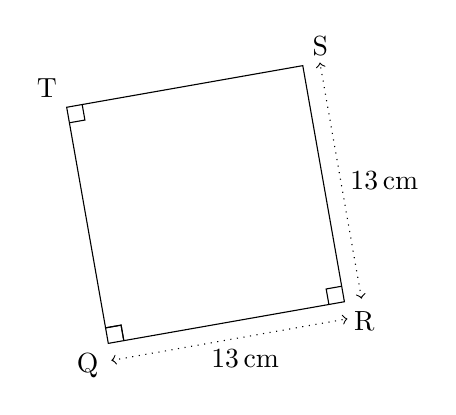
\begin{tikzpicture}[scale=1.1, baseline=(current bounding box.north)]
    \begin{scope}[rotate=10]
        % Draw square
        \draw (0,0) coordinate (Q) --
              ++(2.768,0) coordinate (R) --
              ++(0,2.768) coordinate (S) --
              ++(-2.768,0) coordinate (T) -- cycle;

        % Right angle markers
        \foreach \p/\q/\r in {T/Q/R,Q/R/S,S/T/Q,T/Q/R} {
            \pic [draw, -, angle radius=0.2cm] {right angle=\p--\q--\r};
        }

        % Vertex LABELS
        \foreach \p/\l in {Q/below left,R/below right,S/above right,T/above left} {
            \node[\l] at (\p) {\p};
        }

        % Dotted arrows shifted away from edges
        % Horizontal side (A-B), shifted down
        \draw[<->, dotted]
            ($(Q) + (0,-0.2cm)$) -- ($(R) + (0,-0.2cm)$)
            node[midway,below, xshift=2mm] {13\,cm};

        % Vertical side (B-C), shifted right
        \draw[<->, dotted]
            ($(R) + (0.2cm,0)$) -- ($(S) + (0.2cm,0)$)
            node[midway,right] {13\,cm};
    \end{scope}
\end{tikzpicture}
\end{minipage}%
\hfill
\begin{minipage}{.4\textwidth}
  \begin{align*}
  \text{Area} &= l^2 \\
  \text{Area} &= 13 \,\text{cm} \times 13 \,\text{cm} \\
  \text{Area} &= 169 \,\text{cm}^2
  \end{align*}
\end{minipage}
\par\vspace{1cm}\begin{minipage}{0.55\textwidth}
  \refstepcounter{minipagecount}
  \noindent{(\theminipagecount)}\quad
  \begin{tikzpicture}[scale=1.1, baseline=(current bounding box.north)]
    \begin{scope}[rotate=0]
        % Draw square
        \draw (0,0) coordinate (E) --
              ++(2.756,0) coordinate (F) --
              ++(0,2.756) coordinate (G) --
              ++(-2.756,0) coordinate (H) -- cycle;

        % Right angle markers
        \foreach \p/\q/\r in {H/E/F,E/F/G,G/H/E,H/E/F} {
            \pic [draw, -, angle radius=0.2cm] {right angle=\p--\q--\r};
        }

        % Vertex LABELS
        \foreach \p/\l in {E/below left,F/below right,G/above right,H/above left} {
            \node[\l] at (\p) {\p};
        }

        % Dotted arrows shifted away from edges
        % Horizontal side (A-B), shifted down
        \draw[<->, dotted]
            ($(E) + (0,-0.2cm)$) -- ($(F) + (0,-0.2cm)$)
            node[midway,below, xshift=2mm] {19\,cm};

        % Vertical side (B-C), shifted right
        \draw[<->, dotted]
            ($(F) + (0.2cm,0)$) -- ($(G) + (0.2cm,0)$)
            node[midway,right] {19\,cm};
    \end{scope}
\end{tikzpicture}
\end{minipage}%
\hfill
\begin{minipage}{.4\textwidth}
  \begin{align*}
  \text{Area} &= l^2 \\
  \text{Area} &= 19 \,\text{cm} \times 19 \,\text{cm} \\
  \text{Area} &= 361 \,\text{cm}^2
  \end{align*}
\end{minipage}
\par\vspace{1cm}\begin{minipage}{0.55\textwidth}
  \refstepcounter{minipagecount}
  \noindent{(\theminipagecount)}\quad
  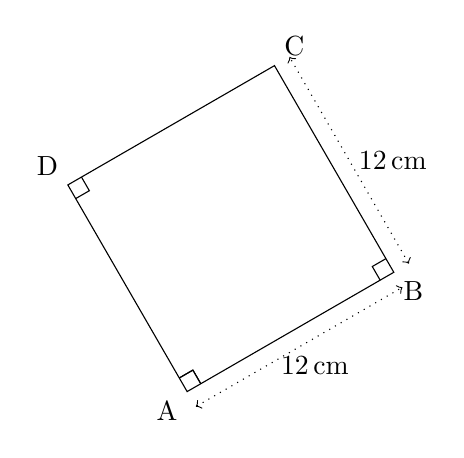
\begin{tikzpicture}[scale=1.1, baseline=(current bounding box.north)]
    \begin{scope}[rotate=30]
        % Draw square
        \draw (0,0) coordinate (A) --
              ++(2.755,0) coordinate (B) --
              ++(0,2.755) coordinate (C) --
              ++(-2.755,0) coordinate (D) -- cycle;

        % Right angle markers
        \foreach \p/\q/\r in {D/A/B,A/B/C,C/D/A,D/A/B} {
            \pic [draw, -, angle radius=0.2cm] {right angle=\p--\q--\r};
        }

        % Vertex LABELS
        \foreach \p/\l in {A/below left,B/below right,C/above right,D/above left} {
            \node[\l] at (\p) {\p};
        }

        % Dotted arrows shifted away from edges
        % Horizontal side (A-B), shifted down
        \draw[<->, dotted]
            ($(A) + (0,-0.2cm)$) -- ($(B) + (0,-0.2cm)$)
            node[midway,below, xshift=2mm] {12\,cm};

        % Vertical side (B-C), shifted right
        \draw[<->, dotted]
            ($(B) + (0.2cm,0)$) -- ($(C) + (0.2cm,0)$)
            node[midway,right] {12\,cm};
    \end{scope}
\end{tikzpicture}
\end{minipage}%
\hfill
\begin{minipage}{.4\textwidth}
  \begin{align*}
  \text{Area} &= l^2 \\
  \text{Area} &= 12 \,\text{cm} \times 12 \,\text{cm} \\
  \text{Area} &= 144 \,\text{cm}^2
  \end{align*}
\end{minipage}
\par\vspace{1cm}

\end{document}
